\chapter{Genomic Location Effect}\label{gle}

The tendency for mutations to occur in closed \gls{chromatin} regions has been reported both in cancer and other mutagenesis processes \citep{Polak2015,Prendergast2007ChromatinGenome}. This is hypothetically because closed chromatin regions, despite being less exposed to mutagens, are harder for repair systems to reach \citep{Prendergast2007ChromatinGenome,Teng1997ExcisionSequences, Morse2002PhotoreactivationCerevisiae}. Based on the premise that different cell-types harbour different chromatin structures \citep{Kundaje2015IntegrativeEpigenomes}, it is reasonable to expect that when developed into tumours, mutations are allocated differently between different cell-types. This chapter shows further evidence, through a G-test of independence and the \gls{or} statistic, that in cancers, mutations do tend to occur in closed rather than open chromatin regions, with the exception of breast adenocarcinoma and rectal cell carcinoma. The degree at which this phenomenon occurs varies across cancer types. In addition, the chapter also uses the \gls{bootstrap} to confirm that \gls{gle} alone, without the chromatin status input, are significantly different in different cancers. 

\section{Mutation location is influenced by chromatin status}
My analyses of GLE were in accordance with the observation that mutations tend to locate in closed chromatin regions. Figure \ref{fig:mutation_density} shows the distribution of mutations on chromosome 12 for four cancers, the rest can be found in Figure \ref{fig:apdx_mutation_density} of the appendix. The green DHS bars near the bottom of the plots are hypersensitive regions, so chromatin is open at regions with dense DHS bars. The choice to display chromosome 12 was arbitrary. By visualisation alone, it can already be seen that mutation density tends to peak at regions with less dense DHS bars, indicating a bias towards closed chromatin regions. This pattern is particularly strong in Skin-Melanoma and Liver-HCC, and less obvious in Kidney-RCC. It is also worth noting that the chromatin structures are different for different cancers. Looking at the density by itself, we could see a diversity in how mutations are distributed, supporting the potential of GLE in discriminating cancers. Unsurprisingly, there are certain conserved patterns for the cancers, which hypothetically correspond to important characteristics of human cells. For example, the level of mutations tend to drop around position 5$\times 10^7$, at which chromatin is closed for all cell types.  

\begin{figure}[ht!]
    \begin{subfigure}{.5\textwidth}
    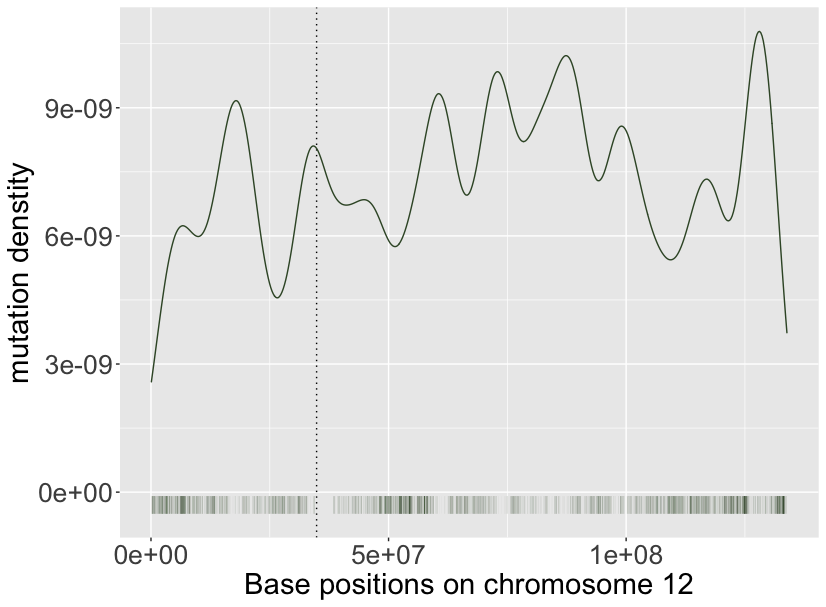
\includegraphics[width=\linewidth,height=0.7\textwidth]{graphics/mutdistribution_Skin-Melanoma.png}
    \caption{Skin-Melanoma}
    \label{fig:density_skin}
    \end{subfigure}
    ~
    \begin{subfigure}{.5\textwidth}
    
    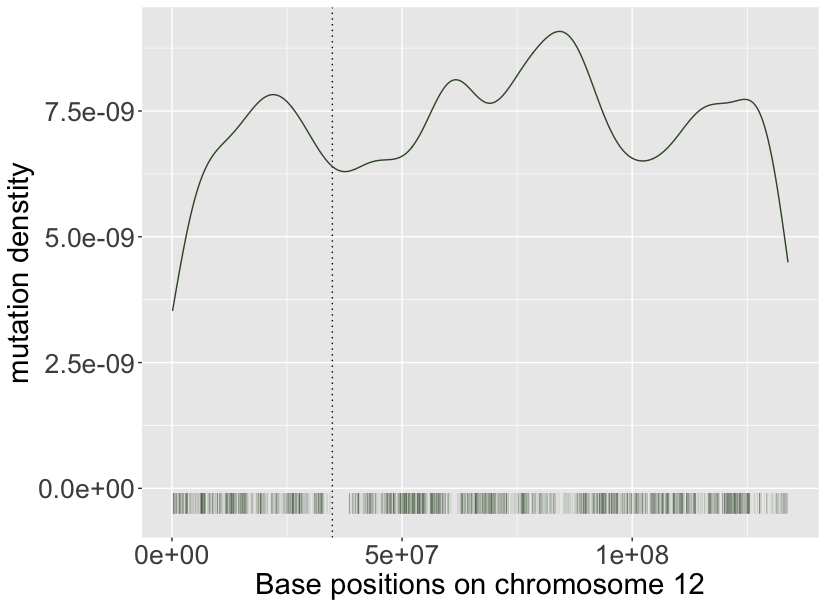
\includegraphics[width=\linewidth,height=0.7\textwidth]{graphics/mutdistribution_Kidney-RCC.png}
    \caption{Kidney-RCC}
    \label{fig:density_kidney}
    \end{subfigure} \\
    \vspace{0.5cm}
    
    \begin{subfigure}{.5\textwidth}
    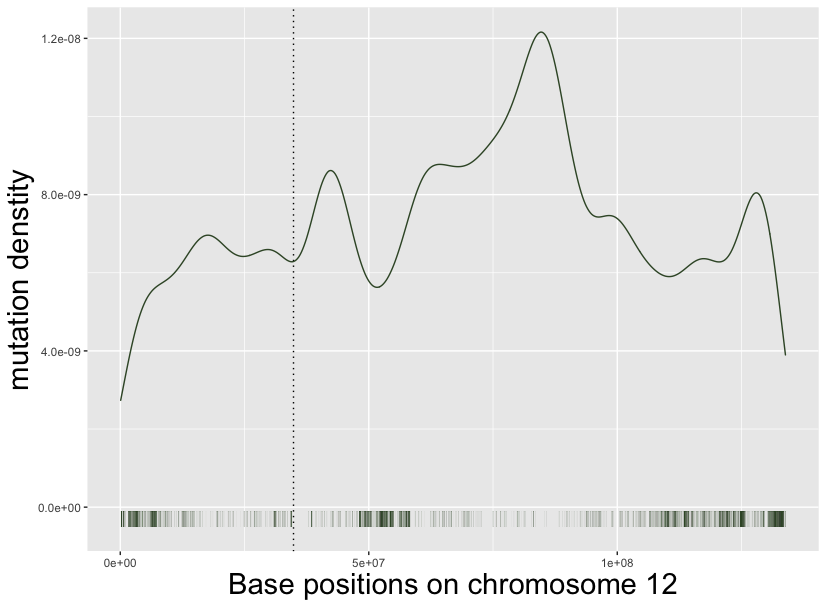
\includegraphics[width=\linewidth,height=0.7\textwidth]{graphics/mutdistribution_Liver-HCC.png}
    \caption{Liver-HCC}
    \label{fig:density_liver}
    \end{subfigure}
    ~
    \begin{subfigure}{.5\textwidth}
    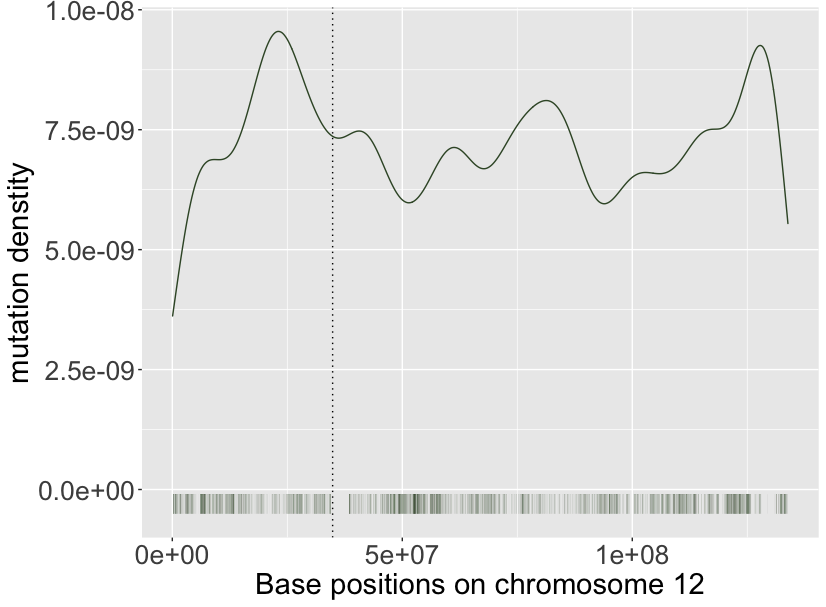
\includegraphics[width=\linewidth,height=0.7\textwidth]{graphics/mutdistribution_Panc-AdenoCA.png}
    \caption{Panc-AdenoCA}
    \label{fig:density_panc_adenoca}
    \end{subfigure} \\
    \caption{\textbf{Mutations tend to be found in closed chromatin regions.} Different cancers differ in the distribution of mutations across the genome. Here chromosome 12 is shown. (a) Skin-Melanoma (b) Kidney-RCC (c) Liver-HCC (d) Panc-AdenoCA, the other cancers are shown in Figure \ref{fig:apdx_mutation_density}. The shaded bars below the x-axis indicate open chromatin regions, the gaps indicate closed chromatin regions of the original cell types. The vertical dotted line indicates the position of the centromere.}
    \label{fig:mutation_density}
\end{figure}

\subsection{Open and closed chromatin regions have significantly different mutation rates}
Having visualised the tendency of mutation location, I performed a G-test of independence to see whether a formal hypothesis test can confirm that there is a difference in how mutations are distributed between open and closed chromatin regions. The p-values estimated from this were adjusted by Bonferroni multiple test correction and shown in Table \ref{tab:g-test}; the raw inputs can be found in Appendix \ref{apdx:g-test}. Most cancers had significantly different mutation rates between open and closed chromatin regions, except CNS-PiloAstro and Panc-Endocrine. Note that these two cancers had small to modest number of mutations. While no direct correlation between p-values and number of mutations could be detected, no cancers with less than 1 million mutations gave a p-value $>10^{-100}$. Our conclusion remains that mutation location is definitely not random between open and closed chromatin regions, but this implies the impact of mutation load on the power of the test.

% latex table generated in R 4.1.0 by xtable 1.8-4 package
% Tue Oct 19 08:53:20 2021
\begin{table}[h]
\centering
\caption{\textbf{The chance of mutations occurring are significantly different between closed and open regions for most cancers.} The table presents }
\label{tab:g-test}
\begin{tabular}{lrr}
  \toprule
 \textbf{Disease} & \textbf{$\hat{p}$-value} & \textbf{Number of mutations} \\ 
  \hline
 Bone-Osteosarc & 5.66 $\times 10^{-35}$ & 166845 \\ 
 Breast-AdenoCa & 1.33 $\times 10^{-10}$ & 713855 \\ 
 CNS-Medullo & 2.46 $\times 10^{-34}$ & 209997 \\ 
 CNS-PiloAstro & 1.00 & 22020 \\ 
 Kidney-RCC & 2.60 $\times 10^{-06}$ & 531886 \\ 
 Liver-HCC & $<10^{-100}$ & 3321521 \\ 
 Lymph-BNHL & $<10^{-100}$ & 1124881 \\ 
 Lymph-CLL & $<10^{-100}$ & 226242 \\ 
 Panc-AdenoCA & $<10^{-100}$ & 1675781 \\ 
 Panc-Endocrine & 8.82 $\times 10^{-02}$ & 258564 \\ 
 Prost-AdenoCA & 5.49 $\times 10^{-90}$ & 1000496 \\ 
 Skin-Melanoma & $<10^{-100}$ & 7770980 \\ 
   \bottomrule
\end{tabular}
\end{table}

\subsection{Mutations are biased towards closed regions, with variation}

\begin{figure}[h!]
    \centering
    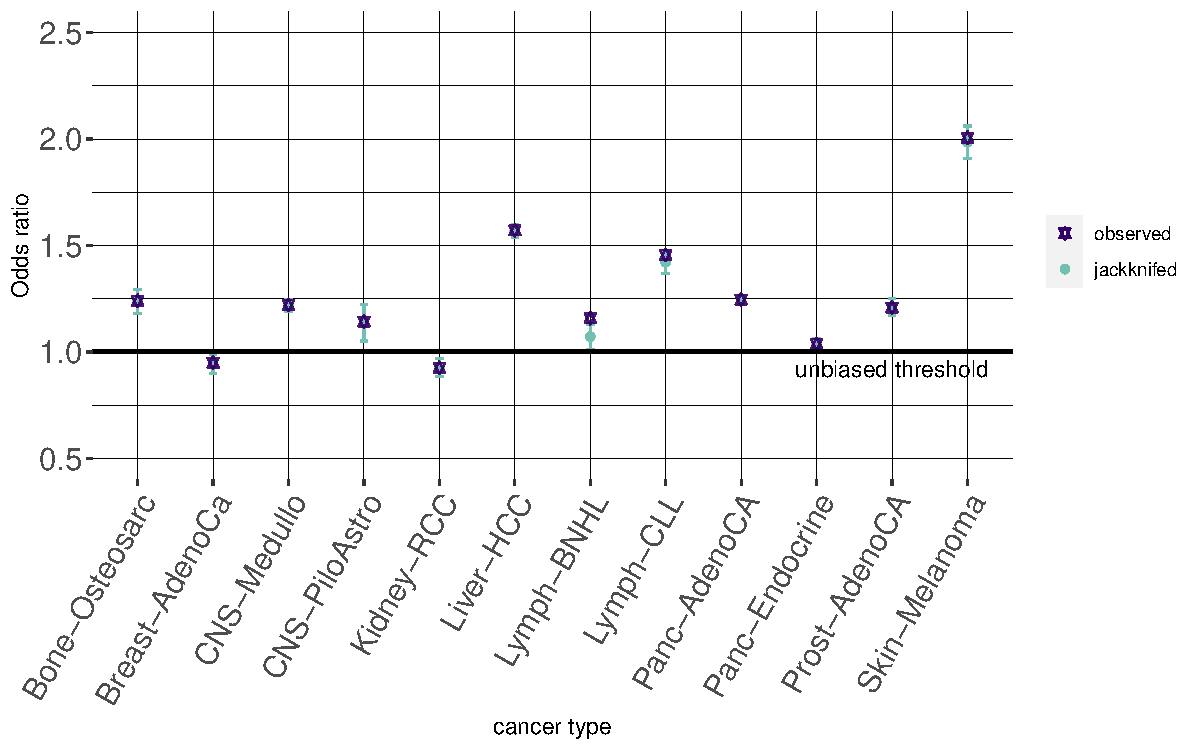
\includegraphics[scale=0.8]{graphics/jackknife_OR.pdf}
    \caption{\textbf{Mutations tend to occur in closed chromatin regions according to the odds ratio ($OR$) statistic}. $OR>1$ indicates a bias towards towards closed regions, and $OR<1$ indicates the opposite. Error bars are the standard errors of the jackknifed sample. The green circles are the means of the jackknifed pseudo-values. The purple stars are the observed $OR$.}
    \label{fig:or_jackknifed}
\end{figure}


\section{GLE is significantly different for different cancers}